\documentclass[12pt,a4paper]{report}

\usepackage[spanish]{babel}
\usepackage[utf8]{inputenc}
\usepackage{dad}

\title{Desarrollo de Aplicaciones Distribuidas: \\ Registrador de juegos}
\author{Rafael Gálvez-Cañero, Andreas Gerstmayr}
\date{Iteración 3 - 9 de Abril de 2015} % delete this line to display the current date



%%% BEGIN DOCUMENT
\begin{document}
\maketitle
\tableofcontents
\listoffigures
\listoftables

\pagenumbering{arabic}

% Esto representa la primera iteración (capítulo), información general
\chapter{Datos generales}

\section{Miembros del grupo}

\begin{table}[htdp]
\begin{center}
\begin{tabular}{|l|l|l|c|}
\hline
\textbf{Apellidos}&\textbf{Nombre}&\textbf{Correo-e}&\textbf{Grupo}\\
\hline
Gálvez-Cañero&Rafael&\href{mailto:galvesband@gmail.com}{galvesband@gmail.com}&18\\
Gerstmayr&Andreas&\href{mailto:andreas.gerstmayr@gmail.com}{andreas.gerstmayr@gmail.com}&18\\
\hline
\end{tabular}
\end{center}
\caption{Miembros del grupo}
\label{tab:miembros}
\end{table}%


\section{Descripción del sistema}

\begin{itemize}
\item \textbf{Tipo de sistema distribuido}:
\item \textbf{Nombre del proyecto}: Plataforma de juegos, Game Register
\item \textbf{Breve descripción}: Sub-sistema para registrar sesiones de juego e información asociada.
\end{itemize}

\subsection{Funcionalidad observable}

\begin{itemize}
\item Registrar el inicio y el término de todas las sesiones de juego.
\item Visualizar el historial de juegos.
\item Visualizar qué jugadores juegan en este momento.
\end{itemize}

\subsection{Servicios ofrecidos}
\begin{itemize}
\item Servicio de Registro: Capacidad de aceptar la información de una sesión de juego.
\item Servicio de Historial: Ofrece métodos para consultar el historial de sesiones.
\item Servicio de Sesiones Online: Muestra una lista de jugadores actualmente en activo.
\end{itemize}

\subsection{Servicios demandados}
\begin{itemize}
\item Servicio X: breve descripción. Fecha aproximada a partir de la que se necesitará (si se conoce).
\item Servicio Y: idem.
\end{itemize}

\section{Direcciones de descarga y planificación}

\begin{table}[htdp]
\begin{center}
\begin{tabular}{|c|c|}
\hline
\textbf{Código fuente}&\url{https://repositorio.informatica.us.es/svn/lq3vqrtzfnh2nx9yhpk}\\
\hline
\multicolumn{2}{|c|}{\textbf{Planificación temporal}}\\
\hline
Iteración 1&17/02/2015\\
Iteración 2&01/03/2015\\
Iteración 3&15/03/2015\\
Iteración 4&05/04/2015\\
Iteración 5&19/04/2015\\
Iteración 6&10/05/2015\\
Iteración 7&24/05/2015\\
Entrega Final&07/06/2015\\
\hline
\end{tabular}
\end{center}
\caption{Datos generales del trabajo en grupo}
\label{tab:datosgenerales}
\end{table}%

\section{Seguimiento}

\begin{table}[htdp]
\begin{center}
\begin{tabular}{|c|c|c|c|c|c|c|c|c|c|c|c|}
\cline{2-10}
\multicolumn{1}{c}{}&\multicolumn{9}{|c|}{\textbf{Iteración}}&\multicolumn{2}{c}{}\\
\hline
\textbf{Estudiante}&1&2&3&4&5&6&7&8&Final&Total&Pond.\\
\hline
Rafael Gálvez-Cañero&5&5&5&5&5&5&5&5&5&\textbf{40}&1\\
Andreas Gerstmayr&5&5&5&5&5&5&5&5&5&\textbf{40}&1\\
\hline
Total&30&30&30&30&30&30&30&30&\multicolumn{2}{c}{}\\
\cline{1-9}
\end{tabular}
\end{center}
\caption{Tabla de seguimiento}
\label{tab:seguimiento}
\end{table}%


% Segunda iteración (capítulo), diagramas UML de clases y despliegue
\chapter{Modelado}

\section{Análisis del sistema}
 \begin{center}
  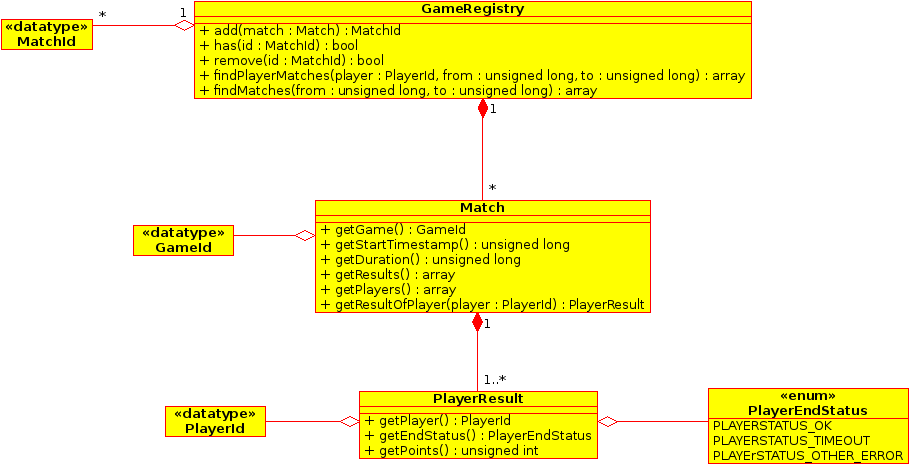
\includegraphics[scale=0.6]{./class_diagram.png}
  % class_diagram.png: 0x0 pixel, 300dpi, 0.00x0.00 cm, bb=
 \end{center}


\section{Arquitectura del sistema}
\begin{figure}[h]
 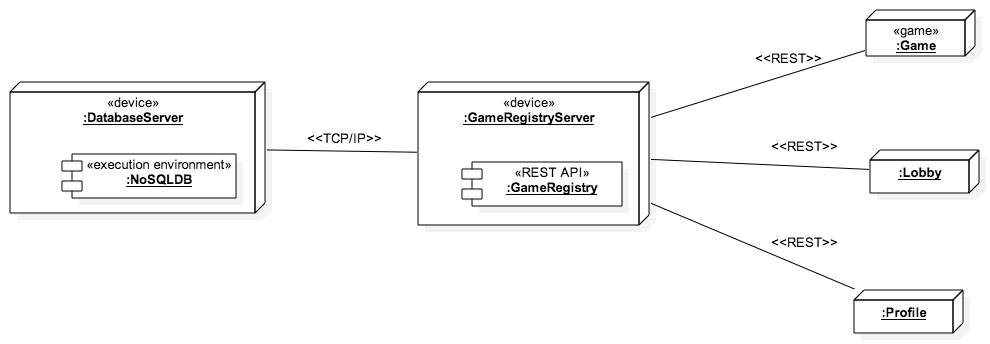
\includegraphics[scale=0.5]{diagrams/deployment_diagram.png}
 \caption{Modelo de despliegue del sistema}
 \label{fig:arquitectura}
\end{figure}


% Tercera iteración (capítulo)
\chapter{Iteración 3}
\section{Objetivos de iteración}
\begin{itemize}
  \item Integración de Gradle 
  \item Servidor dockerizado
  \item Estructura inicial del Cliente vertx.
\end{itemize}

\section{Gradle}
\emph{Gradle} es un gestor de construcción especialmente indicado para proyectos
Java y con soporte para \emph{Groovy}, \emph{Vertx} y \emph{Maven}.

Ha sido integrado mediante el wrapper \texttt{gradlew} que permite utilizar Gradle sin
instalarlo de forma global en el sistema de desarrollo. La primera vez que se
lanza descargará todas las bibliotecas necesarias.

En el archivo \textbf{Readme.md} hay información básica sobre como construir el
proyecto. Algunos comandos útiles:

\begin{itemize}
 \item Para \textbf{construir} el proyecto: \texttt{\$ ./gradlew clean modZip}
 \item Para \textbf{lanzar} el servidor en la máquina local: \texttt{\$ ./gradlew runMod -i}
 \item Para lanzar los \textbf{tests}: \texttt{\$ ./gradlew clean test}
 \item Para preparar el proyecto para un \textbf{entorno de desarrollo}:
    \begin{itemize}
      \item Eclipse: \texttt{\$ ./gradlew eclipse}
      \item IDEA: \texttt{\$ ./gradlew idea}
    \end{itemize}
\end{itemize}

\section{Dockerización}
\emph{Docker} es una tecnología que permite utilizar contenedores sobre \emph{Linux} para
ejecutar procesos de forma aislada y con un runtime reproducible.

Nuestro proyecto proporciona un archivo \textbf{Dockerfile} con las instrucciones necesarias
para construir el contenedor de la aplicación. Además, el archivo \textbf{Readme.md} contiene
información sobre el procedimiento para lanzar el proyecto en \emph{Docker}.

% Cuarta iteracion
\chapter{Iteración 4}
\section{Objetivos de iteración}
\begin{itemize}
  \item Integración de MongoDB (como contenedor docker) 
  \item Cliente más avanzado. Servidor estructurado en Servicio / Controlador.
\end{itemize}

\section{Integración de MongoDB}
\emph{MongoDB} es una base de datos no relacional (\emph{NoSQL}) basada en documentos y
que utiliza \emph{JSon} como formato de intercambio de información.

La integración se ha realizado mediante un contenedor \emph{Docker} de forma que tanto el
desarrollo como el despliegue es fácilmente reproducible.

El servidor GameRegistry necesita una instancia de \emph{MongoDB} funcionando para funcionar.
La integración, realizada mediante el módulo \emph{Vertx} llamado \emph{MongoDB persistor}, depende
de un archivo de configuración para obtener los datos relativos a la conexión con \emph{MongoDB}.
Cambiando los parámetros de este archivo de configuración es posible hacer que el servidor
GameRegistry se conecte a una u otra instancia de \emph{MongoDB}.

Hay que tener en cuenta que el contenedor de \emph{MongoDB} utiliza un \emph{Volumen} (un espacio
de almacenamiento ``externo'' al contenedor que persiste de un lanzamiento a otro). A menudo es
conveniente configurar el lanzamiento del contenedor de \emph{MongoDB} de forma que dicho volumen
corresponda a una carpeta del host:

\texttt{\$ docker run -v [local path]:/data/db/ --name mongo-server mongo:3.0.1}

donde \texttt{local path} es la ruta a una carpeta del host que será utilizada por \emph{Docker}
para montar la carpeta \texttt{/data/db} en el contenedor de \emph{Docker}. De este modo
los archivos relativos a la base de datos de \emph{MongoDB} quedan fuera del contenedor y es
posible examinarlos de forma externa o hacer copias de seguridad fácilmente.

\subsection{MongoDB y desarrollo}
Para desarrollar el servidor GameRegistry o lanzarlo de forma local fuera de un entorno
de contenedores \emph{Docker} tan solo es necesario obtener una instancia de \emph{MongoDB}
a la que se pueda conectar y un archivo de configuración con la información necesaria para
la conexión.

En el archivo \textbf{Readme.md} hay información básica sobre cómo conseguir una instancia
de MongoDB utilizando \emph{Docker}, que resulta a menudo más conveniente que instalar una
instancia local del mismo.

Hay que tener en cuenta que los contenedores de \emph{Docker} por defecto no exponen los puertos
al host. Las instrucciones básicas para lanzar \emph{MongoDB} como contenedor para desarrollo 
serían:

\begin{itemize}
 \item Descargar el contenedor (sólo la primera vez): \texttt{\$ docker pull mongo:3.0.1}
 \item Lanzar la instancia de \emph{MongoDB} exponiendo el puerto al host: 
       \texttt{\$ docker run -P mongo:3.0.1}
 \item Modificar la configuración de GameRegistry si es necesario en el archivo \emph{conf.json}
 \item Lanzar el servidor GameRegistry: \texttt{\$ ./gradlew runMod -i}
\end{itemize}

\subsection{MongoDB y despliegue}
El \emph{Dockerfile} que describe cómo construir el contenedor de nuestro servidor GameRegistry
ha sido actualizado para integrar un archivo de configuración separado dedicado al contenedor 
llamado \emph{conf-docker.json}. Este archivo contiene la configuración necesaria (mínima) para
poder conectar con un servidor \emph{MongoDB} que corre en una máquina llamada \texttt{mongo-server}.
Esto resulta conveniente en un entorno \emph{Docker} enlazando ambos contenedores. Por ejemplo:

\begin{itemize}
 \item Descargar el contenedor de \emph{MongoDB} (sólo la primera vez): \texttt{\$ docker pull mongo:3.0.1}
 \item Lanzar la instancia de \emph{MongoDB} sin exponer puertos al host y nombrando la instancia del contenedor:
       \texttt{\$ docker run --name mongo-server mongo:3.0.1}
 \item Construir el contenedor para nuestro servidor: \texttt{\$ docker build -t distributedsystems/gameregistry .}
 \item Lanzar el contenedor de GameRegistry enlazándolo con el de la instancia de \emph{Docker} de forma
       que compartan la pila de red (y puedan así comunicarse), exponiendo el puerto de GameRegistry en el host:
       \texttt{\$ docker run -p 8080:8080 --link mongo-server:mongo-server distributedsystems/gameregistry}
\end{itemize}

\subsection{Distinción de dominio, controlador y servicio}
\begin{description}
  \item[Dominio] \hfill \\
  Clases POJO con el mismo esquema de la base de datos.
  \item[Controlador] \hfill \\
  Manejar los requisitos y respuestas y comunicar con el servicio.
  \item[Servicio] \hfill \\
  La lógica de negocio. Almacenar las sessiones en el base de datos.
\end{description}

\section{Diagrama de paquetes}
\begin{center}
 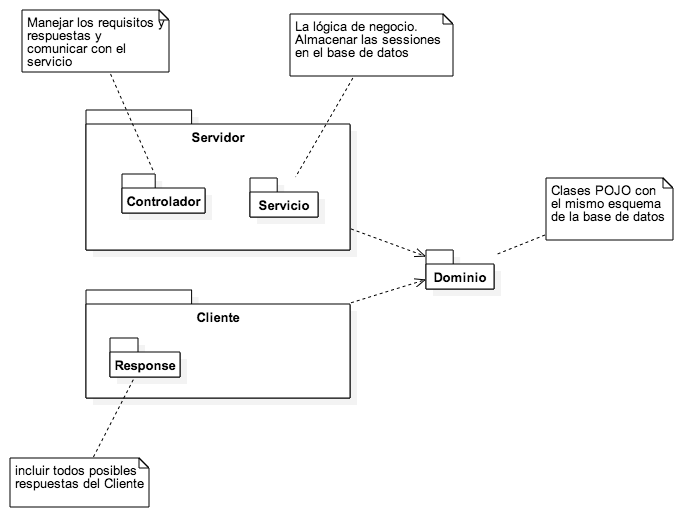
\includegraphics[scale=0.6]{diagrams/package_diagram.png}
\end{center}

\chapter{Iteracion 5}
\section{Objetivos de iteración}
\begin{itemize}
  \item Implementación inicial de API
  \item Primeros tests.
  \item Despliegue Azure plataforma
  \item ¿Integración contínua?
\end{itemize}

\section{Diagrama de despliegue}
\begin{center}
 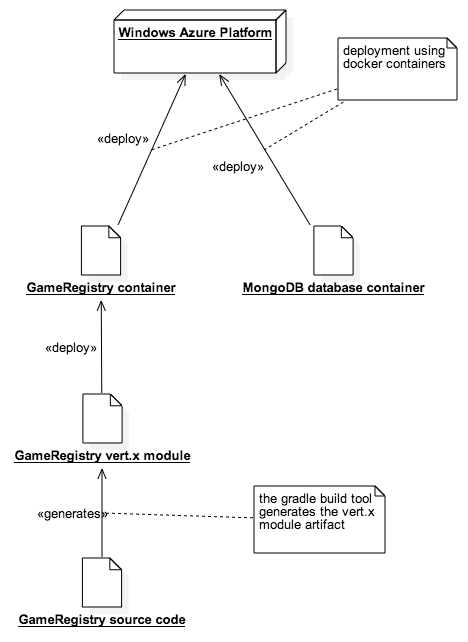
\includegraphics[scale=0.6]{diagrams/docker_deployment_diagram.png}
\end{center}
 
\chapter{Iteracion 6}
\section{Objetivos de iteración}
Final testing.

\chapter{Iteracion 7}
\section{Objetivos de iteración}
Subir a repositorio Maven.

\end{document}
\appendix

\chapter{Documentación de API MyService}

Aquí el texto que se considere necesario.
